\documentclass[a4paper,11pt,cours]{nsi} % COMPILE WITH DRAFT
\geometry{margin=2cm}
\usepackage[]{fontawesome5}

\usetikzlibrary{trees}

\setcounter{chapter}{3} % 1 de moins que le num de chapitre

\setlength{\columnseprule}{0pt}
\setlength{\columnsep}{1cm}

\chapter{Fonction logarithme népérien}

\begin{document}

\section{Fonction réciproque}
\begin{propriete}[ et définition : Fonction réciproque]
	Soit $f$ une fonction continue et strictement monotone sur un intervalle $I$, à valeurs dans un intervalle $J$.\\
	Il existe une fonction définie sur $J$ et à valeurs dans $I$, appelée \textbf{fonction réciproque de $f$} et notée $f^{-1}$ telle que $$\text{pour tous réels } x\in I \text{ et } y\in J,\text{ l'égalité }\ f(x)=y\ \text{ est équivalente à }\ x=f^{-1}(y).$$
\end{propriete}

\begin{exemple}[]
	\dleft{11.8cm}
	{
		La fonction $f$ définie sur $I=\fio{0}{+\infty}$ par $\ f(x)=x^2\ $ est dérivable donc \textbf{continue} sur $I$ et strictement croissante sur $I$.\\
		Elle prend ses valeurs dans $J=\fio{0}{+\infty}$.\\

		Pour tous $x\in I$ et $y\in J, \quad y=x^2\quad \iff \quad \sqrt{y}=x$.\\

		Donc la fonction réciproque de $f$ est la fonction racine carrée.
        $$\text{Pour tout } x\in\fio{0}{+\infty},\ f^{-1}(x)=\sqrt{x}.$$
	}
	{
		\def\xmin{-1} \def\ymin{-1}\def\xmax{4}\def\ymax{5}
		\def\F{\x^2}
		\begin{tikzpicture}[scale=.7]
			\clip (\xmin,\ymin) rectangle (\xmax,\ymax);
			\draw[fill = white] (\xmin,\ymin) rectangle (\xmax,\ymax);
			\repereal{\xmin}{\ymin}{\xmax}{\ymax}
			\draw[color=UGLiOrange,thick,domain=0:3,smooth,variable=\x] plot ({\x},{\F});
			\draw[color=UGLiOrange] (2,4) node[above left]{$y=x^2$};
			\draw[color=olive] (4,4) node[left]{$y=x$};
			\draw[color=olive,thick,domain=0:\xmax,smooth,variable=\x] plot ({\x},{\x});
			\draw[color=UGLiRed,thick,domain=0:\xmax,smooth,variable=\x] plot ({\x},{\x^0.5});
			\draw[color=UGLiRed] (4,1.7) node[below left]{$y=\sqrt{x}$};
			%\pointc{1}{2.718}{}{$e$}{$A$}
			
		\end{tikzpicture}	
	}
\end{exemple}

\section{Fonction logarithme népérien}

On a vu que la fonction exponentielle est une fonction continue et strictement croissante sur $\R$.\\

\dleft{9.5cm}{
    De plus $\ \lim\limits_{x\to-\infty}e^x=0\quad$ et $\quad \lim\limits_{x\to+\infty}e^x=+\infty$.
    \begin{center}
        \begin{tikzpicture}
        \tkzTabInit[color,lgt=2,espcl=4]
        {$x$/.7,$x\mapsto e^x$ /2}
        {$-\infty$, $+\infty$}
        \tkzTabVar{-/$0$,+/$+\infty$}
        \end{tikzpicture}
    \end{center}
    La fonction exponentielle admet donc une fonction réciproque définie sur $\oio{0}{+\infty}$. 
}
{
    \def\xmin{-5} \def\ymin{-1}\def\xmax{3}\def\ymax{5}
		\def\F{exp(\x)}
		\begin{tikzpicture}[scale=.8]
			\clip (\xmin,\ymin) rectangle (\xmax,\ymax);
			\draw[fill = white] (\xmin,\ymin) rectangle (\xmax,\ymax);
			\repereal{\xmin}{\ymin}{\xmax}{\ymax}
			\draw[color=UGLiOrange,thick,domain=\xmin:3,smooth,variable=\x] plot ({\x},{\F});
			\draw[color=UGLiOrange] (2,4.5) node{\courbe{\exp}};
			%\draw[color=olive] (4,4) node{(T)};
			%\draw[color=olive,thick,domain=\xmin:\xmax,smooth,variable=\x] plot ({\x},{\x});
			\pointc{1}{2.718}{}{$e$}{$A$}
			
		\end{tikzpicture}
}
\newpage

\begin{definition}[]
    On appelle fonction \textbf{logarithme népérien} et on note $\ln$ la fonction réciproque de la fonction exponentielle.\\
    Ainsi pour tous $x\in\oio{0}{+\infty}$ et $y\in\R, \quad \ln(x)=y\quad$ équivaut à $\quad x=e^y$.
\end{definition} 

\dleft{10cm}{
    \begin{enumerate}[label=\textbullet]
        \item $e^0=1\quad$ donc $\quad \ln 1=0$;
        \item $e^1=e\quad$ donc $\quad \ln e=1$.
    \end{enumerate}
    \begin{center}
        \tabstyle[UGLiGreen]
 \begin{tabular}{|c|c|c|c|c|c|}
 \hline
 \ccell $x$ & $\ e^{-1}\ $ & \hspace*{.2cm}$1$\hspace*{.2cm} & \hspace*{.2cm}$2$ \hspace*{.2cm}& \hspace*{.2cm}$e$\hspace*{.2cm} & $e^3$ \\\hline
 \ccell $\ln x$ & $-1$ & $0$ & $\ln 2$ & $1$ & \hspace*{.2cm}$3$\hspace*{.2cm} \\\hline
 \end{tabular}
    \end{center}
    
    \begin{propriete}[]
        Dans un reprère orthonormé, les courbes représentatives des fonctions logarithme népérien et exponentielle sont symétriques par rapport à la droite d'équation $y=x$.
    \end{propriete}
}
{
    \def\xmin{-2} \def\ymin{-3}\def\xmax{5}\def\ymax{5}
		\def\F{exp(\x)}
		\begin{tikzpicture}[scale=.8]
			\clip (\xmin,\ymin) rectangle (\xmax,\ymax);
			\draw[fill = white] (\xmin,\ymin) rectangle (\xmax,\ymax);
			\repereal{\xmin}{\ymin}{\xmax}{\ymax}
			\draw[color=UGLiOrange,thick,domain=\xmin:3,smooth,variable=\x] plot ({\x},{\F});
			\draw[color=UGLiOrange] (2,4.5) node{\courbe{\exp}};
			\draw[color=olive] (3.5,3.5) node[below right]{$y=x$};
			\draw[color=olive,thick,domain=\xmin:\xmax,smooth,variable=\x] plot ({\x},{\x});
            \draw[color=olive,thick,domain=\xmin:\xmax,smooth,variable=\x] plot ({\x},{\x});
			\pointc{1}{2.718}{}{$e$}{}
			\draw[color=UGLiRed,thick,domain=0.01:\xmax,smooth,variable=\x] plot ({\x},{ln(\x)});
            \draw[color=UGLiRed] (4,1) node{\courbe{\ln}};
            \pointc{2.718}{1}{$e$}{}{}
		\end{tikzpicture}
}


\begin{encadrecolore}{Conséquences de la définition}{UGLiDarkBlue}
    \begin{enumerate}[label=\textbullet]
        %\item La fonction $\ln$ est définie, continue et strictement croissante sur $\oio{0}{+\infty}$ ;
        \item Pour tout réel $x,\ \ln(e^x)=x$ ;
        \item Pour tout réel $x>0,\ e^{\ln x}=x$ ;
    \end{enumerate}
\end{encadrecolore}

\begin{propriete}[]
    La fonction $\ln$ est strictement croissante sur $\oio{0}{+\infty}$.
\end{propriete}

\dleft{9cm}{
    \begin{demonstration}
        Soient $a$ et $b$ deux réels tels que $0<a<b$.\\
        On a donc $\quad e^{\ln a}<e^{\ln b}$.\\
        Or la fonction exponentielle est strictement croissante sur $\R$ donc :
        $$\ln a < \ln b$$
        On a ainsi prouvé que pour tous $0<a<b,$\\
        $\ln a< \ln b.$
    \end{demonstration}
}
{
    \def\xmin{-1.5} \def\ymin{-3}\def\xmax{8}\def\ymax{3}
		\begin{tikzpicture}[scale=.7]
			\clip (\xmin,\ymin) rectangle (\xmax,\ymax);
			\draw[fill = white] (\xmin,\ymin) rectangle (\xmax,\ymax);
			\repereal{\xmin}{\ymin}{\xmax}{\ymax}
			\pointc{2}{.693}{$a$}{$\ln a$}{}
			\draw[color=UGLiRed,thick,domain=0.01:\xmax,smooth,variable=\x] plot ({\x},{ln(\x)});
            \draw[color=UGLiRed] (7,2) node[above]{\courbe{\ln}};
            \pointc{6}{1.792}{$b$}{$\ln b$}{}
		\end{tikzpicture}
}

\begin{encadrecolore}{Conséquences}{UGLiDarkBlue}
    Pour tous réels strictement positifs $a$ et $b$ :
    \begin{enumerate}[label=\textbullet]
        \item $\ln a=\ln b \quad \iff \quad a=b$ ;
        \item $\ln a<\ln b \quad \iff \quad 0<a<b$ ;
        \item $\ln a>0 \quad \iff \quad a>1$ ;
        \item $\ln a<0 \quad \iff \quad 0<a<1$ ;
    \end{enumerate}
\end{encadrecolore}

\section{Propriétés algébriques du logarithme népérien}
\begin{propriete}[ : Relation fonctionnelle]
    Pour tous réels strictement positifs $a$ et $b$, $\qquad \ln(a\times b)=\ln a +\ln b$.
\end{propriete}

\begin{demonstration}
    Soient $a$ et $b$ deux réels strictement positifs.\\ 
    $e^{\ln (a\times b)}=a\times b\quad$ et $\quad e^{\ln a +\ln b}=e^{\ln a} \times e^{\ln b}=a \times b$.\\
    On a donc $\quad e^{\ln (a\times b)}=e^{\ln a + \ln b} \quad$ d'où $\quad \ln(a\times b)=\ln a + \ln b$.
\end{demonstration}

\begin{exemple}[s]
    \begin{enumerate}[label=\textbullet]
        \item $\ln 10 =\ln(2\times 5)=\ln 2+\ln 5$
        \item Pour $x>0, \quad \ln(2x)=\ln 2+\ln x$
        \item Pour $x>0, \quad \ln(x^2)=\ln x + \ln x=2\ln x$
    \end{enumerate}

\end{exemple}

\dleft{12cm}{
    \begin{encadrecolore}{Un peu d'histoire}{UGLiPurple}
        La fin du 16$^{\text{e}}$ siècle est l'époque des grands voyages maritimes et de la découverte des lois régissant le mouvement des planètes. Les mesures astronomiques, nécessaires pour la navigation, impliquent des calculs compliqués. Les multiplications, divisions et extractions de racines sont particulièrement pénibles à la main.\\[.5em]
        Après de longues années de travail, la mathématicien écossais \textbf{John Napier} établit, en 1614, une table appelée « table de logarithmes » qui permet, grâce à la relation fonctionnelle précédente, de remplacer le calcul d'une multiplication par une addition.
    \end{encadrecolore}
}
{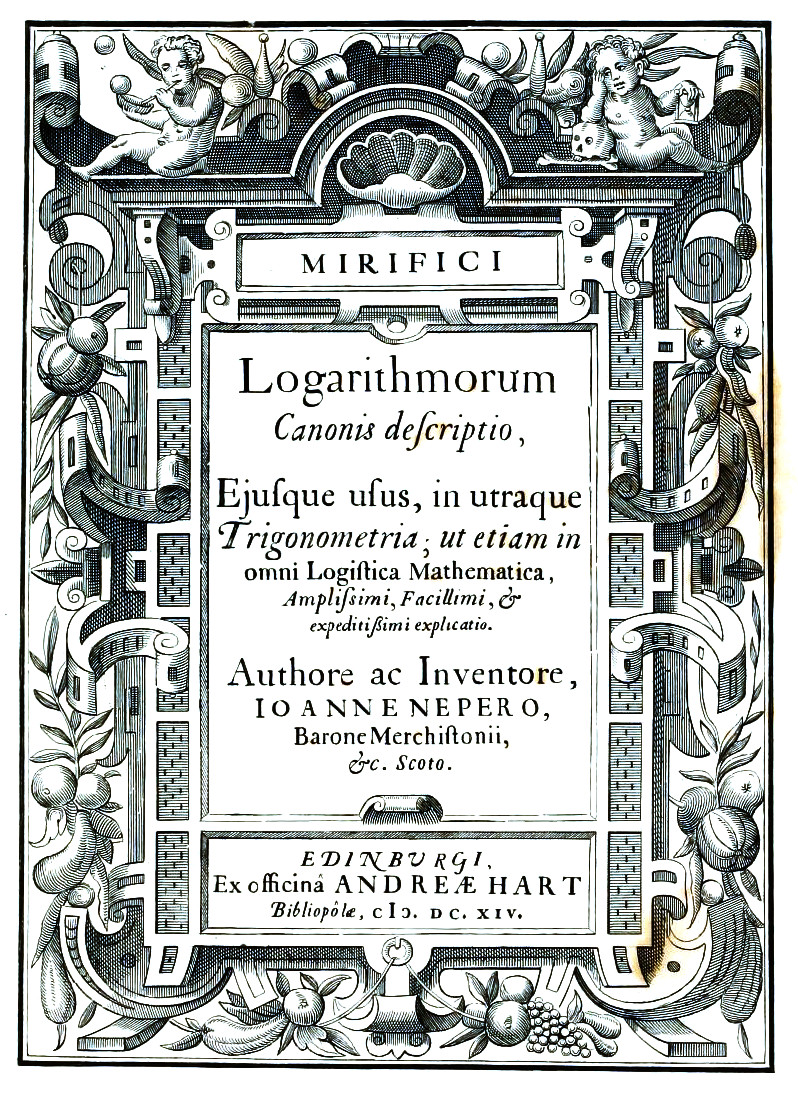
\includegraphics[width=4cm]{Logarithms_book_Napier.jpg}}

\begin{propriete}[s]
    Soient $a$ et $b$ deux réels strictement positifs et $n$ un entier.
    \begin{multicols}{4}
        \begin{enumerate}[label=\textbullet]
            \item $\ln \dfrac{1}{a}=-\ln a$
            \item $\ln \dfrac{a}{b}=\ln a-\ln b$
            \item $\ln a^n=n\ln a$
            \item $\ln \sqrt{a}=\dfrac{1}{2}\ln a$
        \end{enumerate}
    \end{multicols}
\end{propriete}

\begin{demonstration}
    \begin{enumerate}[label=\textbullet]
        \item $a\times \dfrac{1}{a}=1\quad$ donc $\quad \ln 1=\ln\left(a\times\dfrac{1}{a}\right)=\ln a +\ln \dfrac{1}{a}\quad$ d'où $\quad 0=\ln a+\ln \dfrac{1}{a}\quad$ et ainsi $\quad \ln \dfrac{1}{a}=-\ln a$.
        \item $\ln \dfrac{a}{b}=\ln\left(a\times \dfrac{1}{b}\right)=\ln a +\ln \dfrac{1}{b}=\ln a -\ln b$.
        \item $\ln a^n=\ln \underbrace{a\times a\times \ldots \times a}_{n\text{ facteurs}}=n\ln a$.
        \item $\ln a=\ln \left(\sqrt{a}\right)^2=2\ln \sqrt{a}\quad$ d'où $\quad \dfrac{1}{2}\ln a=\ln \sqrt{a}$.
    \end{enumerate}
\end{demonstration}


\section{Étude de la fonction logarithme népérien}
\begin{propriete}[]
    La fonction $\ln$ est dérivable sur $\oio{0}{+\infty}$ et pour tout $x>0,\quad \ln'(x)=\dfrac{1}{x}$.
\end{propriete}

\begin{demonstration}
    On admet que la fonction $\ln$ est dérivable sur $\oio{0}{+\infty}$.\\
    Soit $f$ la fonction définie sur $\oio{0}{+\infty}$ par $f(x)=e^{\ln x}$.\\
    Soit $x>0$.\\
    On a $ \quad f(x)=x\quad$ donc $\quad f'(x)=1$.\\
    Or $\quad f'(x)=\ln'(x)\times e^{\ln x}=\ln'(x)\times x$.\\
    Donc $\quad \ln'(x)\times x=1\quad$ et $\quad\ln'(x)=\dfrac{1}{x}$.
\end{demonstration}


\begin{propriete}[s (admises)]
    \begin{multicols}{2}
        \begin{enumerate}[label=\textbullet]
            \item $\lim\limits_{x\to 0}\ln x=-\infty$
            \item $\lim\limits_{x\to +\infty}\ln x=+\infty$
        \end{enumerate}
    \end{multicols}
\end{propriete}

\vspace*{0.5cm}

\dleft{10cm}{
    \begin{center}
        \begin{tikzpicture}
            \tkzTabInit[color,lgt=2,espcl=4]
            {$x$/.7,$\ln'x$ /.7,$\ln$ /2}
            {$0$, $+\infty$}
            \tkzTabLine{d,+,}
            \tkzTabVar{ D-/ $-\infty$ , +/ $+\infty$ }
        \end{tikzpicture}
    \end{center}
    L'axe des ordonnées est une \textbf{asymptote verticale} à la courbe représentative de la fonction logarithme népérien.
}
{
    \def\xmin{-1} \def\ymin{-3}\def\xmax{8}\def\ymax{3}
		\begin{tikzpicture}[scale=.7]
			\clip (\xmin,\ymin) rectangle (\xmax,\ymax);
			\draw[fill = white] (\xmin,\ymin) rectangle (\xmax,\ymax);
			\repereal{\xmin}{\ymin}{\xmax}{\ymax}
			\draw[color=UGLiRed,thick,domain=0.01:\xmax,smooth,variable=\x] plot ({\x},{ln(\x)});
            \draw[color=UGLiRed] (7,2) node[above]{\courbe{\ln}};
		\end{tikzpicture}
}

\begin{propriete}[]
    Si $u$ est une fonction dérivable et strictement positive sur un intervalle $I$ , alors la fonction $\ln(u)$ est dérivable sur $I$ et $\quad (\ln u)'=\dfrac{u'}{u}$.
\end{propriete}

\begin{demonstration}
    Soient $a$ et $h$ deux réels de $I$ tels que $a+h\in I$ et $u(a+h)\neq u(a)$.\\
    
    On a $\quad \dfrac{\ln(u(a+h))-\ln(u(a))}{h}=\dfrac{\ln(u(a+h))-\ln(u(a))}{u(a+h)-u(a)}\times \dfrac{u(a+h)-u(a)}{h}$.\\[.5em]
    Or $\quad \lim\limits_{h\to 0}u(a+h)-u(a)=0 \quad$ car $u$ est dérivable donc continue en $a$\\[.5em]
    Donc $\quad \lim\limits_{h\to 0}\dfrac{\ln(u(a+h))-\ln(u(a))}{u(a+h)-u(a)}=\ln'(u(a))=\dfrac{1}{u(a)}$.\\[.5em]
    De plus $\quad \lim\limits_{h\to 0}\dfrac{u(a+h)-u(a)}{h}=u'(a)$.\\
   
    On a donc $\quad \lim\limits_{h\to 0}\dfrac{\ln(u(a+h))-\ln(u(a))}{h}=\dfrac{u'(a)}{u(a)}$.
\end{demonstration}
\end{document}